% !Mode:: "TeX:UTF-8"

\chapter{测试设计与结果}

本项目为8个微服务模块编写了19个测试类，覆盖Controller层、Service层、Mapper层及边界条件测试。测试框架基于JUnit 5 + Mockito + Spring Boot Test，遵循分层测试策略。

\section{测试框架与工具}

\begin{table}[H]
	\centering
	\caption{测试技术栈一览}
	\begin{tabular}{p{5.0cm}p{5.0cm}p{4.0cm}}
		\hline
		\textbf{层面} & \textbf{技术} & \textbf{版本} \\
		\hline
		测试框架 & JUnit 5 (Jupiter) & 5.7.x \\
		Mock框架 & Mockito & 3.9.x \\
		Web层测试 & Spring MockMvc & -- \\
		集成测试 & Spring Boot Test & 2.4.5 \\
		断言库 & JUnit Assertions + Mockito Verify & -- \\
		JSON序列化 & Jackson ObjectMapper & -- \\
		\hline
	\end{tabular}
\end{table}

\section{测试架构设计}

本项目采用四层测试金字塔架构，自底向上覆盖Mapper层、Service层、Controller层和边界场景：

\begin{enumerate}
	\item \textbf{Mapper层测试}（1个测试类）：使用\verb|@SpringBootTest| + \verb|@Transactional|，测试真实数据库的CRUD操作，验证事务自动回滚，确保不污染数据库
	\item \textbf{Service层单元测试}（4个测试类）：使用\verb|@ExtendWith(MockitoExtension.class)|，Mock Mapper和Feign客户端，验证业务逻辑的正确性
	\item \textbf{Controller层测试}（11个测试类）：使用\verb|MockMvcBuilders.standaloneSetup|独立模式，Mock Service层，验证HTTP请求/响应、状态码和JSON结构
	\item \textbf{边界条件测试}（3个测试类）：针对空列表、null值、零数量、重复操作、订单不存在等边界场景，确保系统鲁棒性
\end{enumerate}

\section{测试模块总览}

\begin{table}[H]
	\centering
	\caption{各模块测试统计}
	\begin{tabular}{p{5.5cm}p{1.8cm}p{2.8cm}p{4.0cm}}
		\hline
		\textbf{模块} & \textbf{测试类数} & \textbf{用例数} & \textbf{测试层级} \\
		\hline
		elm-user-server & 1 & 20 & Controller (MockMvc) \\
		elm-business-server & 4 & 28 & Controller + Service + Boundary \\
		elm-food-server & 1 & 2 & Controller (MockMvc) \\
		elm-cart-server & 3 & 15 & Controller + Service + Boundary \\
		elm-order-server & 2 & 15 & Controller + Service (SpringBootTest) \\
		elm-delivery-server & 2 & 7 & Controller + Service (SpringBootTest) \\
		elm-wallet-server & 2 & 6 & Controller + Service \\
		elm-point-server & 4 & 38 & Controller + Service + Mapper + Feign \\
		\hline
		\textbf{合计} & \textbf{19} & \textbf{131} & -- \\
		\hline
	\end{tabular}
\end{table}

\section{用户微服务测试 (elm-user-server)}

\subsection{测试设计}

UserControllerTest（20个用例）基于MockMvc独立模式，Mock UserService和JwtTokenProvider，覆盖以下场景：

\begin{itemize}
	\item \textbf{JWT认证}：验证有效Token返回用户信息（HTTP 200）、无效Token返回401
	\item \textbf{登录认证}：正确凭据返回JWT Token并设置Authorization Header、错误密码返回401
	\item \textbf{密码修改}：验证Token后修改密码成功返回200
	\item \textbf{用户信息更新}：更新本人信息成功（200）、更新他人信息被拒绝（403）
	\item \textbf{用户列表}：获取所有用户列表（200）
	\item \textbf{用户注册}：支持新旧两种注册路径（/api/register 和 /api/users），用户名冲突返回409
	\item \textbf{用户查询}：按用户名查询、按用户ID查询、检查用户存在性
	\item \textbf{边界场景}：缺少必填参数返回400、无Token请求受保护接口返回401
\end{itemize}

\subsection{测试结果}

\begin{figure}[H]
	\centering
	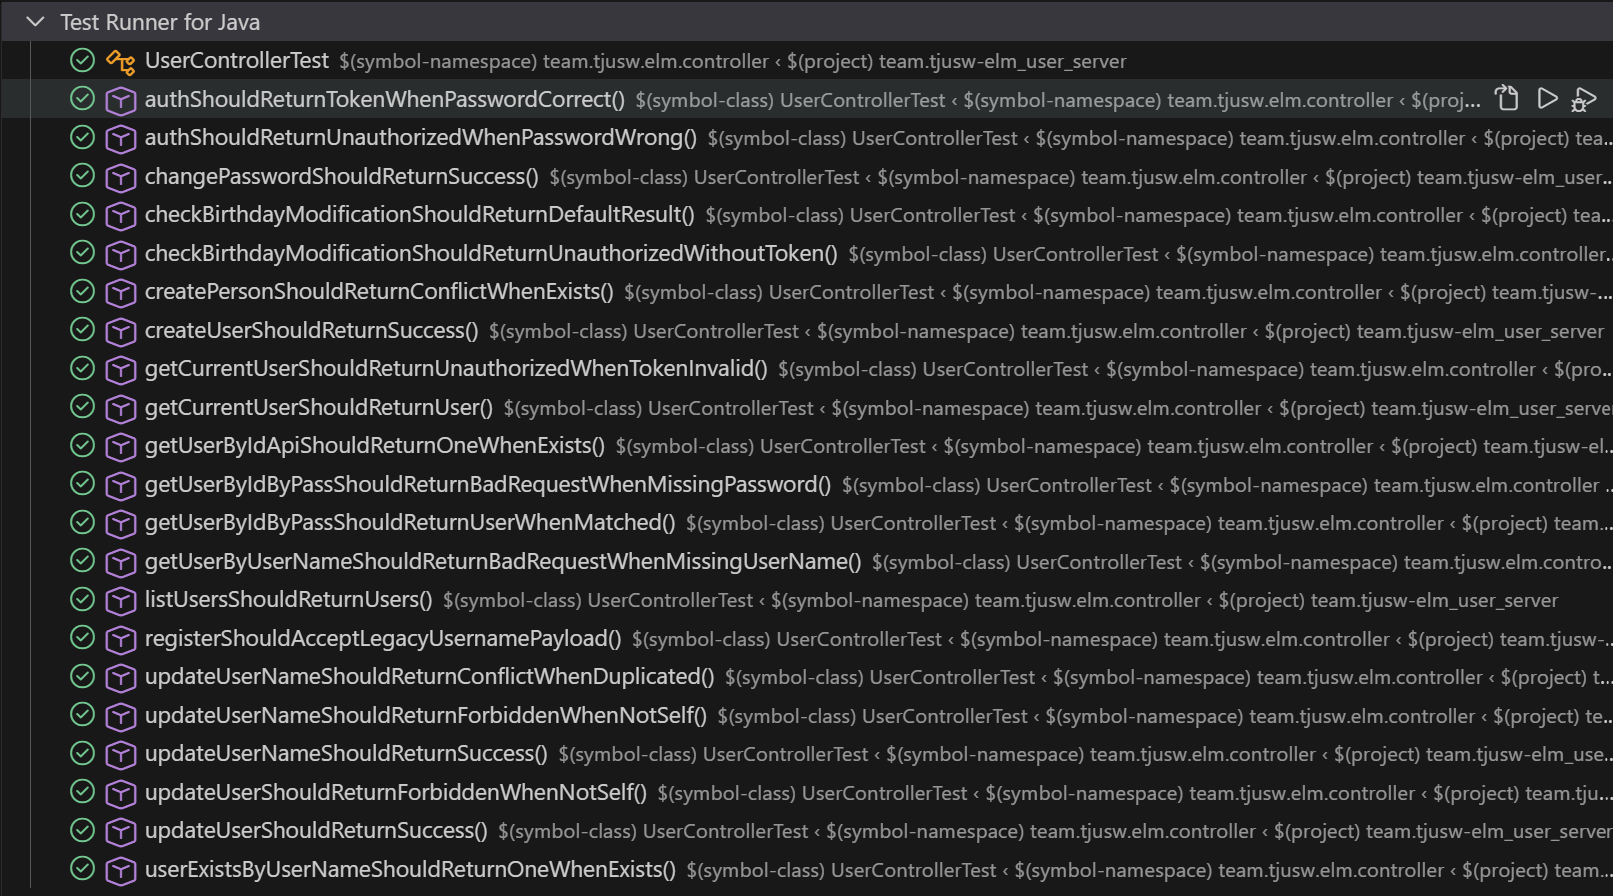
\includegraphics[width=0.85\textwidth,height=0.82\textheight,keepaspectratio]{images/test-user-controller-result.png}
	\caption{用户微服务测试结果}
	\label{fig:test-user-controller}
\end{figure}

\section{商家微服务测试 (elm-business-server)}

\subsection{测试设计}

商家模块包含4个测试类，覆盖Controller和Service两层：

\textbf{BusinessControllerTest}（2个用例）：测试商家创建（POST /businesses，期望返回201和完整商家对象）、商家信息更新（PUT /businesses/\{id\}，验证更新后字段值）。

\textbf{OrderControllerTest}（9个用例）：测试订单创建（POST /orders，期望201）、用户订单列表、商家订单列表、订单详情、订单明细、支付/配送/完成订单状态流转（各期望200）。

\textbf{OrderServiceImplTest}（9个用例）：Mock OrderMapper和RabbitMQSender，测试创建订单（验证saveOrder和saveOrderDetail调用次数）、各类订单查询、更新订单状态（验证RabbitMQ消息发送）、支付/配送/完成订单。

\textbf{OrderServiceImplBoundaryTest}（8个用例）：测试空订单详情创建（验证总金额为0.0）、各类操作在订单不存在时返回0（不发送MQ消息）、查询返回空列表、查询返回null。

\subsection{测试结果}

\begin{figure}[H]
	\centering
	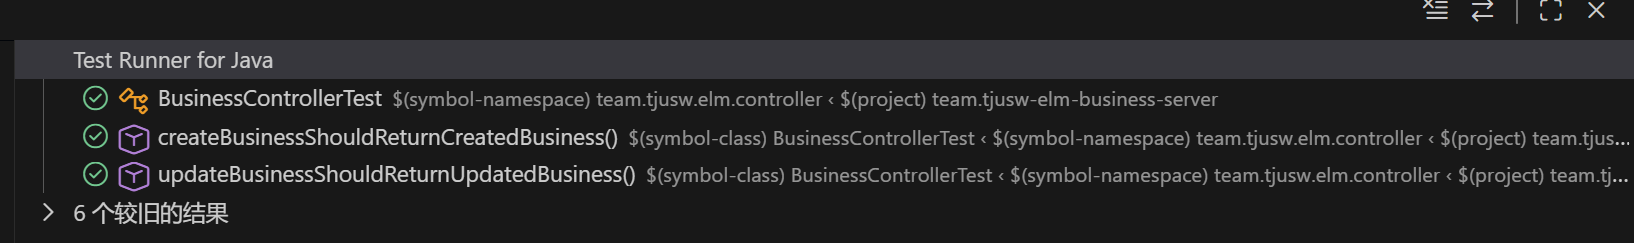
\includegraphics[width=0.85\textwidth,height=0.82\textheight,keepaspectratio]{images/test-business-controller-result.png}
	\caption{商家微服务BusinessController测试结果}
	\label{fig:test-business-controller}
\end{figure}

\begin{figure}[H]
	\centering
	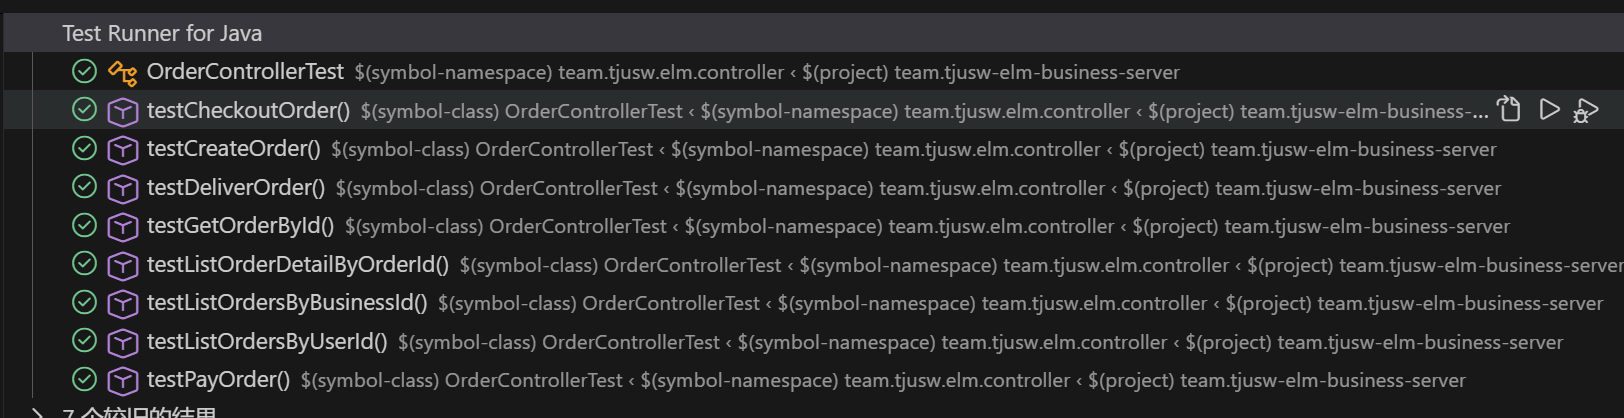
\includegraphics[width=0.85\textwidth,height=0.82\textheight,keepaspectratio]{images/test-order-controller-result.png}
	\caption{商家微服务OrderController测试结果}
	\label{fig:test-order-controller}
\end{figure}

\begin{figure}[H]
	\centering
	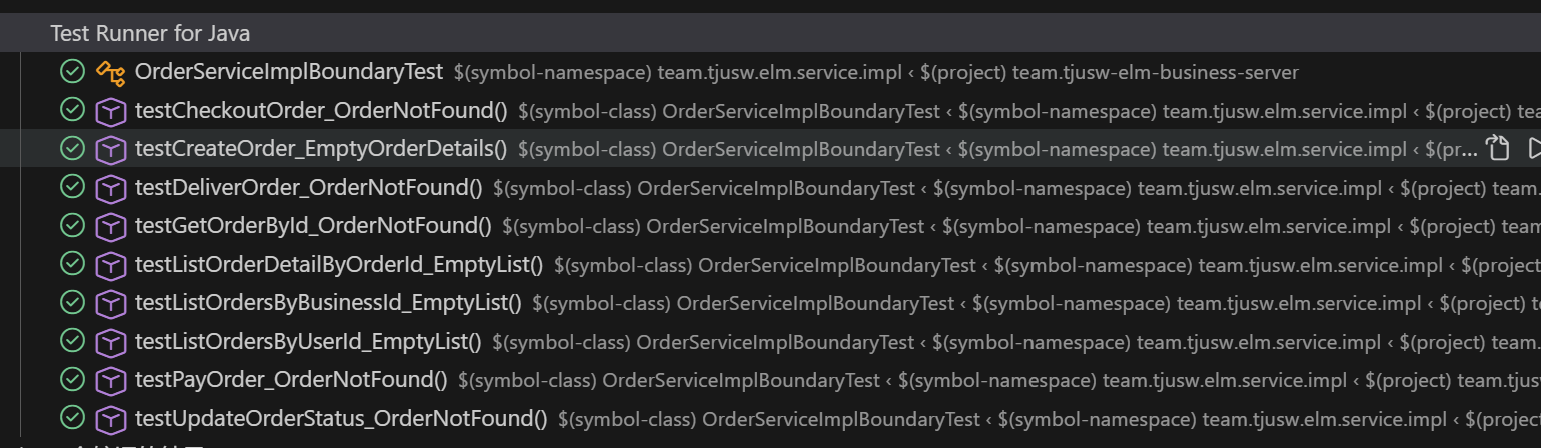
\includegraphics[width=0.85\textwidth,height=0.82\textheight,keepaspectratio]{images/test-order-service-result.png}
	\caption{OrderServiceImpl单元测试结果}
	\label{fig:test-order-service}
\end{figure}


\section{食品微服务测试 (elm-food-server)}

\subsection{测试设计}

FoodControllerTest（2个用例）基于MockMvc，测试食品新增和更新：

\begin{itemize}
	\item \textbf{新增食品}：POST /foods，提交食品对象（含BigDecimal价格），期望返回200且result为true
	\item \textbf{更新食品}：PUT /foods/\{id\}，验证返回对象中的foodId和foodName与预期一致
\end{itemize}

\subsection{测试结果}

\begin{figure}[H]
	\centering
	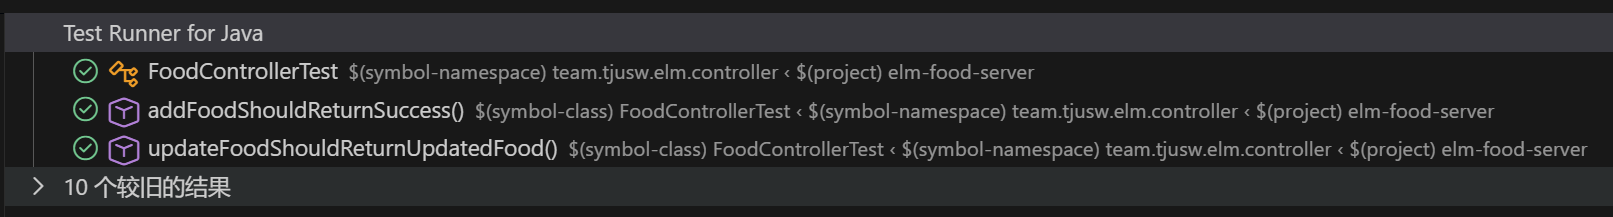
\includegraphics[width=0.85\textwidth,height=0.82\textheight,keepaspectratio]{images/test-food-controller-result.png}
	\caption{食品微服务测试结果}
	\label{fig:test-food-controller}
\end{figure}

\section{购物车微服务测试 (elm-cart-server)}

\subsection{测试设计}

购物车模块包含3个测试类：

\textbf{CartControllerTest}（5个用例）：MockMvc模式测试按用户ID获取购物车列表、按用户和商家获取、按用户和商家和食品删除、新增购物车项（期望201）、更新数量。

\textbf{CartServiceImplTest}（5个用例）：Mock CartMapper，测试新增购物车项——区分"新项插入"（验证insertCart调用、不调updateCart）和"已存在项更新"（验证updateCart调用、不调insertCart）；删除和查询验证返回值正确性和Mock调用次数。

\textbf{CartServiceImplBoundaryTest}（7个用例）：测试空购物车对象新增、零数量商品、删除不存在的项（返回0）、空列表查询、更新不存在的项（返回0）、零数量更新、已存在项零数量覆盖。

\subsection{测试结果}

\begin{figure}[H]
	\centering
	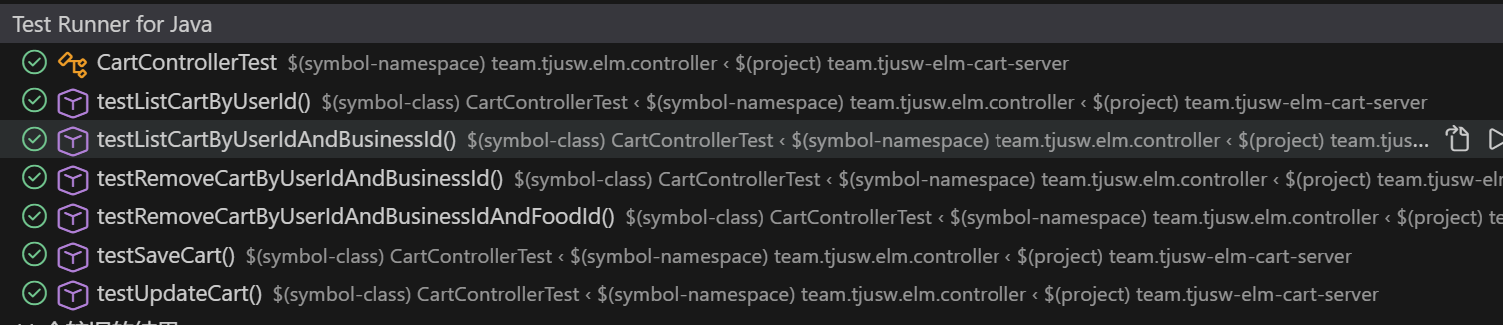
\includegraphics[width=0.85\textwidth,height=0.82\textheight,keepaspectratio]{images/test-cart-controller-result.png}
	\caption{购物车Controller测试结果}
	\label{fig:test-cart-controller}
\end{figure}

\begin{figure}[H]
	\centering
	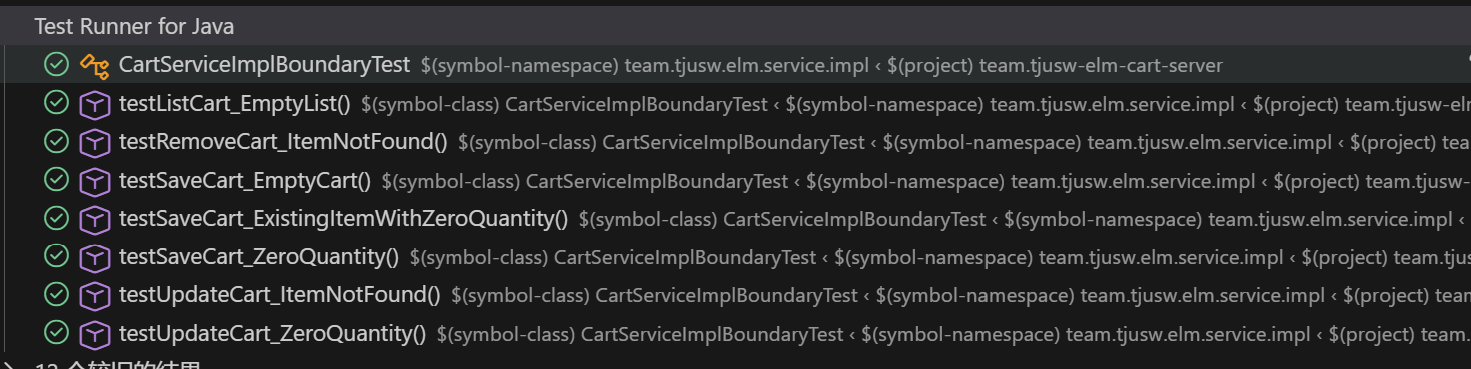
\includegraphics[width=0.85\textwidth,height=0.82\textheight,keepaspectratio]{images/test-cart-service-result.png}
	\caption{CartServiceImpl单元测试结果}
	\label{fig:test-cart-service}
\end{figure}

\begin{figure}[H]
	\centering
	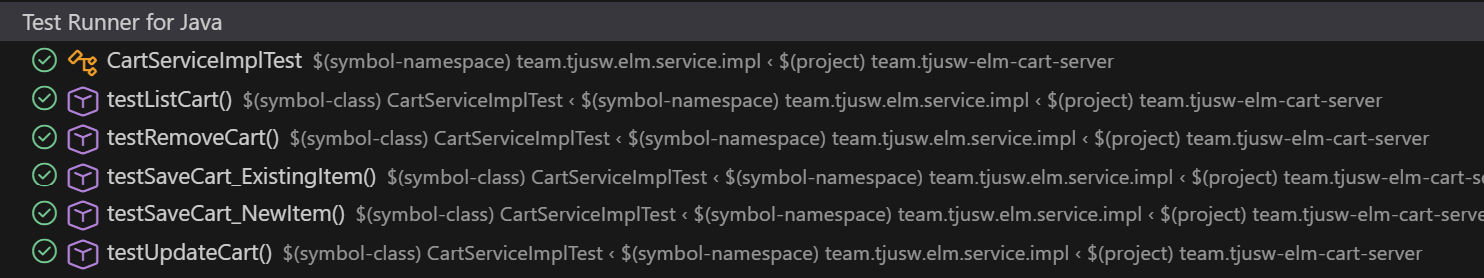
\includegraphics[width=0.85\textwidth,height=0.82\textheight,keepaspectratio]{images/test-cart-boundary-result.png}
	\caption{购物车边界条件测试结果}
	\label{fig:test-cart-boundary}
\end{figure}

\section{订单微服务测试 (elm-order-server)}

\subsection{测试设计}

订单模块包含2个SpringBootTest集成测试类，使用\verb|@MockBean|模拟所有Feign客户端（CartClient、VirtualWalletClient、PointClient、BusinessClient），\verb|@Transactional|自动回滚：

\textbf{OrdersServiceTest}（8个用例）：
\begin{itemize}
	\item 按用户ID和商家ID查询订单列表
	\item 按订单ID查询订单详情（含orderDetailet明细）
	\item 更新订单状态并验证持久化
	\item 创建订单——Mock购物车数据（LinkedHashMap模拟），验证orderDetailet写入正确数量
	\item 虚拟钱包支付成功——Mock完整Feign调用链（获取商家信息→查询余额→查询积分→计算抵扣→转账→积分增减），验证订单状态变为1
	\item 余额不足——验证返回错误码1
	\item 重复支付——第一次返回200，第二次返回3（已支付）
\end{itemize}

\textbf{OrdersControllerTest}（7个用例）：\verb|@SpringBootTest|注入真实Controller，测试Controller层对Service的委托调用。

\subsection{测试结果}

\begin{figure}[H]
	\centering
	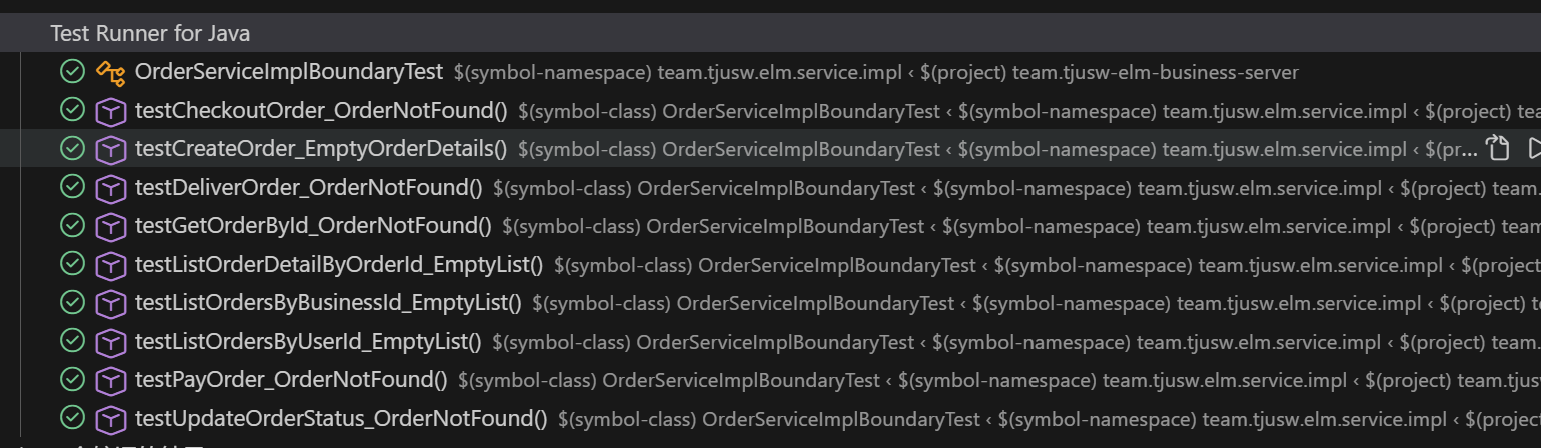
\includegraphics[width=0.85\textwidth,height=0.82\textheight,keepaspectratio]{images/test-order-service-result.png}
	\caption{订单服务OrdersService集成测试结果}
	\label{fig:test-orders-service}
\end{figure}

\section{配送地址微服务测试 (elm-delivery-server)}

\subsection{测试设计}

配送地址模块包含2个SpringBootTest集成测试类：

\textbf{DeliveryAddressControllerTest}（3个用例）：测试查询用户地址列表（验证返回1条记录）、查询单个地址（验证userId一致）、新增地址（期望201和返回1）。

\textbf{DeliveryAddressServiceTest}（4个用例）：测试查询地址列表、新增地址后列表增长、更新地址——验证旧地址失效（valid=0）且新增一条新地址、删除地址——验证valid变为0且有效列表为空。

\subsection{测试结果}

\begin{figure}[H]
	\centering
	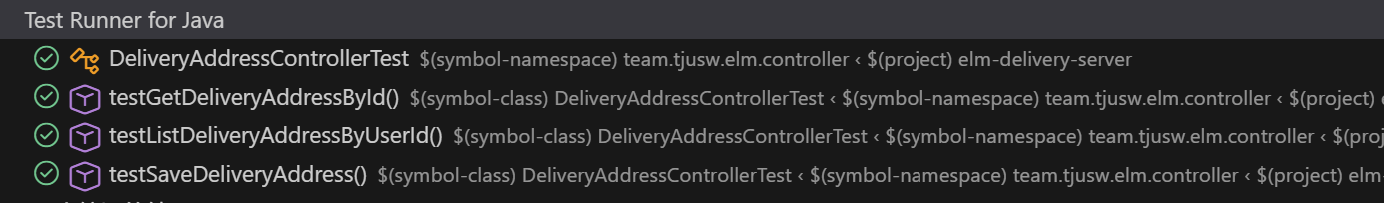
\includegraphics[width=0.85\textwidth,height=0.82\textheight,keepaspectratio]{images/test-delivery-controller-result.png}
	\caption{配送地址Controller测试结果}
	\label{fig:test-delivery-controller}
\end{figure}

\begin{figure}[H]
	\centering
	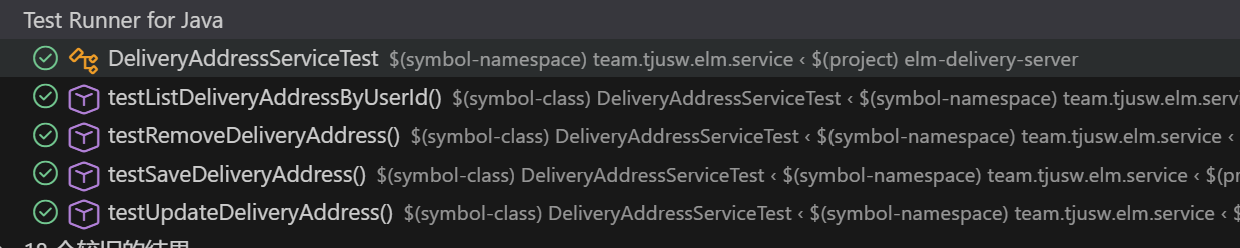
\includegraphics[width=0.85\textwidth,height=0.82\textheight,keepaspectratio]{images/test-delivery-service-result.png}
	\caption{配送地址Service集成测试结果}
	\label{fig:test-delivery-service}
\end{figure}

\section{虚拟钱包微服务测试 (elm-wallet-server)}

\subsection{测试设计}

钱包模块包含2个测试类：

\textbf{VirtualWalletControllerTest}（2个用例）：Mock HttpServletRequest和VirtualWalletService，测试从JWT Token中解析userId并查询钱包余额。使用Base64编码构造无签名JWT（\verb|\{"alg":"none"\}|），验证Controller正确委托Service并返回200和正确userId。

\textbf{VirtualWalletServiceImplTest}（1个用例）：Mock VirtualWalletMapper，测试getBalance方法查询余额（期望返回100.00）。

\subsection{测试结果}

\begin{figure}[H]
	\centering
	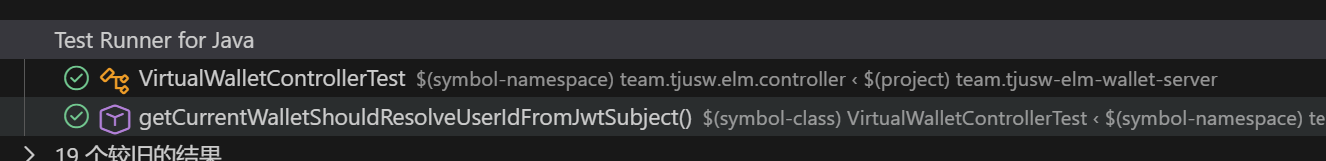
\includegraphics[width=0.85\textwidth,height=0.82\textheight,keepaspectratio]{images/test-wallet-controller-result.png}
	\caption{虚拟钱包Controller测试结果}
	\label{fig:test-wallet-controller}
\end{figure}

\begin{figure}[H]
	\centering
	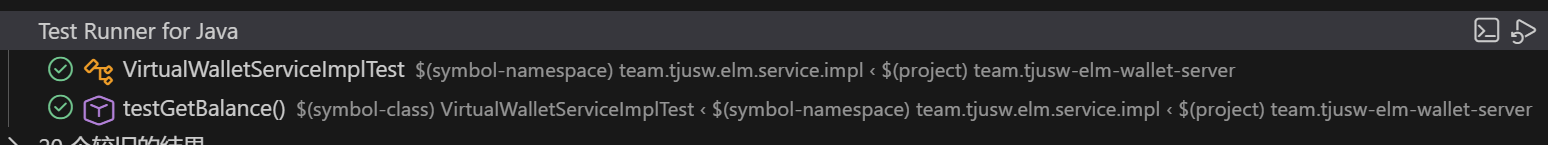
\includegraphics[width=0.85\textwidth,height=0.82\textheight,keepaspectratio]{images/test-wallet-service-result.png}
	\caption{虚拟钱包Service测试结果}
	\label{fig:test-wallet-service}
\end{figure}

\section{积分微服务测试 (elm-point-server)}

\subsection{测试设计}

积分模块是测试覆盖最全面的模块，包含4个测试类：

\textbf{IntegralMapperTest}（7个用例）：\verb|@SpringBootTest|测试真实数据库操作：插入积分记录并验证自增ID、按ID查询、按用户ID时间倒序查询、按状态和过期时间正向排序查询、更新积分状态和剩余数量、按用户和状态汇总可用积分、多用户数据隔离验证。

\textbf{IntegralServiceTest}（17个用例）：测试核心业务逻辑——增加积分、消费积分（成功/积分不足异常）、获取可用积分、首次签到（验证10积分和签到标记）、签到重复（返回0）、订单金额积分计算（取整规则）、评论积分计算（15字阈值，无图5分/有图10分）、积分抵扣计算（100积分=1元，最多抵扣订单金额）、积分明细查询、积分统计（总计/可用/已用/过期）、VIP积分（BASIC/GOLD/PLATINUM/DIAMOND）、活动积分（NEW\_USER/HOLIDAY/UNKNOWN）、生日积分（当天100分/当月10分/非当月0分）、连续签到积分（1-6天1分/7天10分/30天50分）、积分渠道验证、积分过期处理、可用积分详情。

\textbf{IntegralControllerTest}（13个用例）：\verb|@SpringBootTest|测试REST API接口——获取可用积分、手动添加积分、消费积分成功、首次签到、重复签到、评论积分（不满足条件/满足条件无图/满足条件有图）、积分抵扣计算、积分统计、订单发放积分、可用积分详情、积分渠道验证、积分过期处理。

\textbf{PointServiceImplTest}（4个用例）：Mock IntegralService和OrderClient，测试PointService作为Feign代理层正确转发调用——String类型userId的getBalance、earnPointByOrder、deductOrder，以及遗留数字文本userId。

\subsection{测试结果}

\begin{figure}[H]
	\centering
	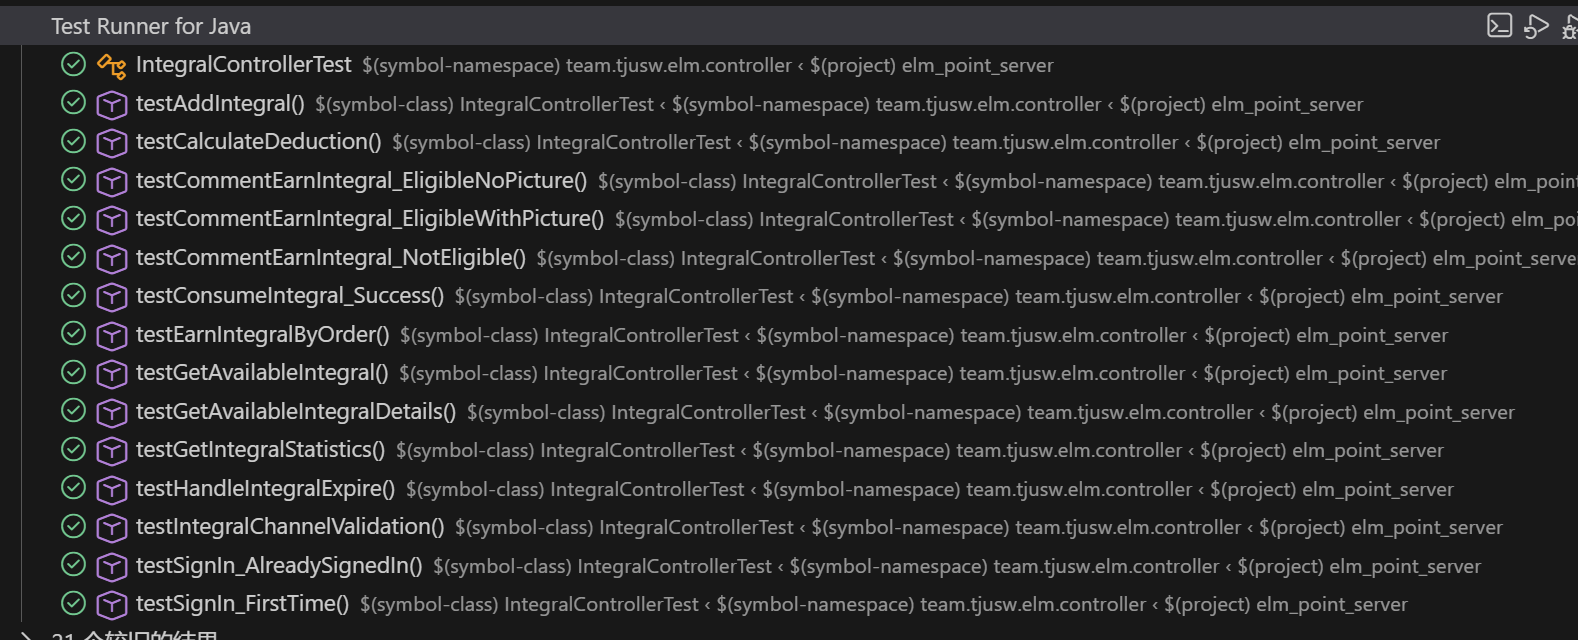
\includegraphics[width=0.85\textwidth,height=0.82\textheight,keepaspectratio]{images/test-integral-controller-result.png}
	\caption{积分Controller测试结果}
	\label{fig:test-integral-controller}
\end{figure}

\begin{figure}[H]
	\centering
	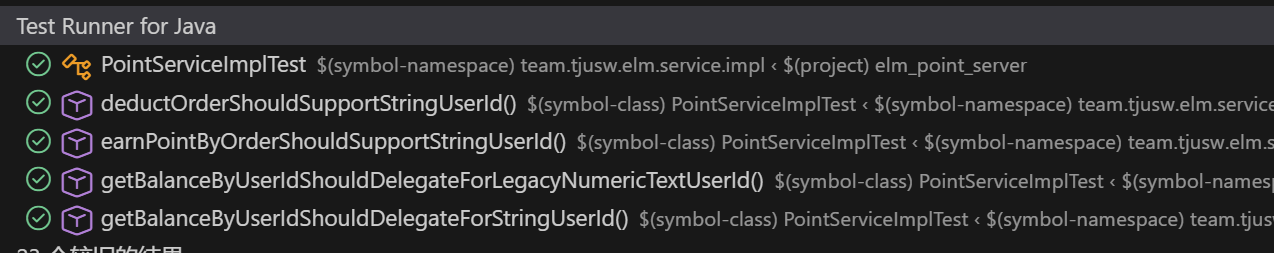
\includegraphics[width=0.85\textwidth,height=0.82\textheight,keepaspectratio]{images/test-integral-service-result.png}
	\caption{积分Service业务逻辑测试结果}
	\label{fig:test-integral-service}
\end{figure}

\begin{figure}[H]
	\centering
	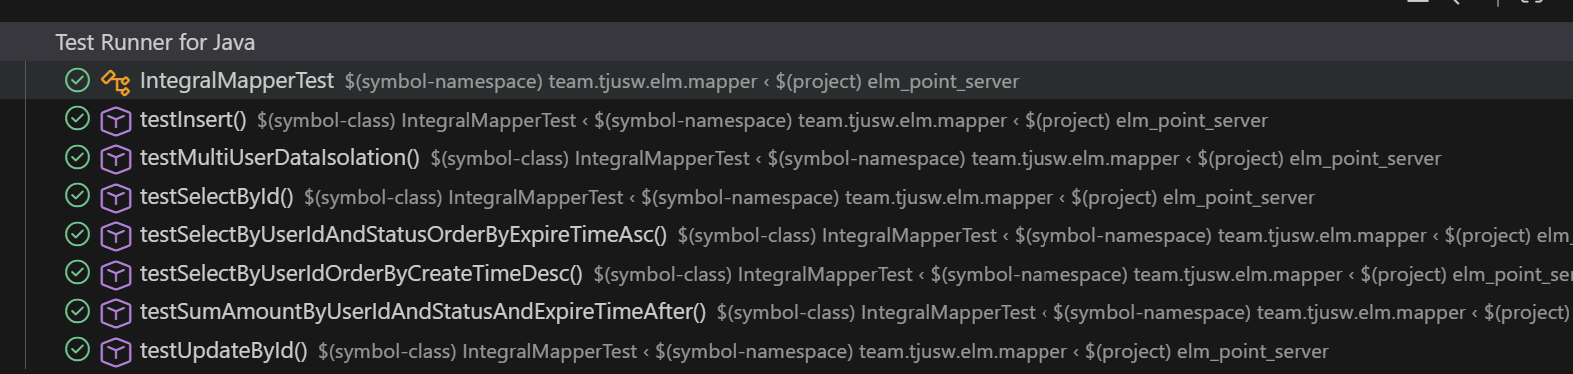
\includegraphics[width=0.85\textwidth,height=0.82\textheight,keepaspectratio]{images/test-integral-mapper-result.png}
	\caption{积分Mapper数据访问层测试结果}
	\label{fig:test-integral-mapper}
\end{figure}

\begin{figure}[H]
	\centering
	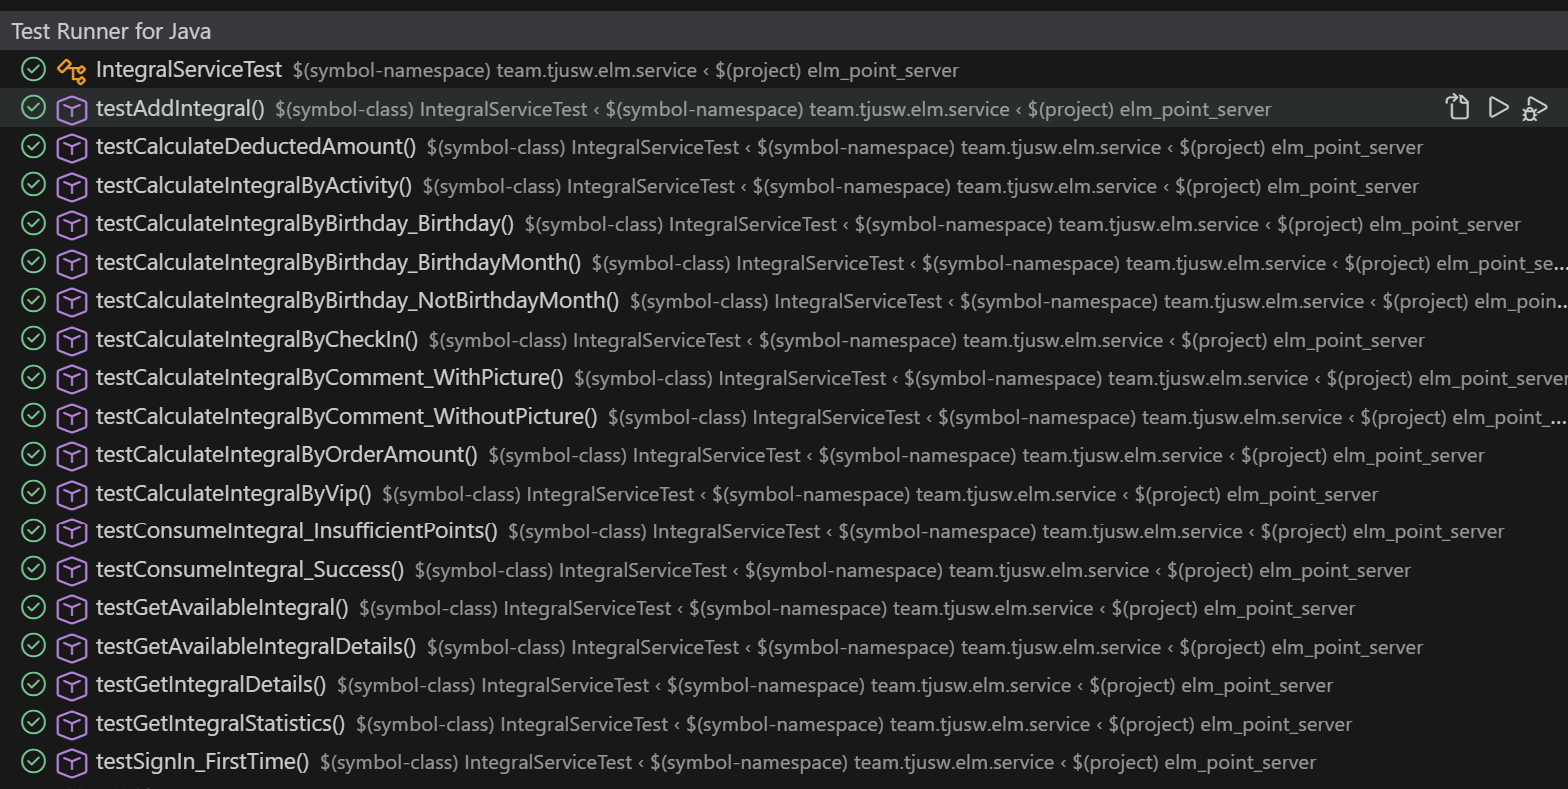
\includegraphics[width=0.85\textwidth,height=0.82\textheight,keepaspectratio]{images/test-point-service-result.png}
	\caption{PointService Feign代理测试结果}
	\label{fig:test-point-service}
\end{figure}

\section{测试覆盖汇总}

\begin{table}[H]
	\centering
	\caption{测试覆盖矩阵}
	\begin{tabular}{p{4.5cm}p{2.5cm}p{2.5cm}p{2.5cm}p{2.5cm}}
		\hline
		\textbf{模块} & \textbf{Controller} & \textbf{Service} & \textbf{Mapper} & \textbf{Boundary} \\
		\hline
		elm-user-server & $\checkmark$ & -- & -- & -- \\
		elm-business-server & $\checkmark$ & $\checkmark$ & -- & $\checkmark$ \\
		elm-food-server & $\checkmark$ & -- & -- & -- \\
		elm-cart-server & $\checkmark$ & $\checkmark$ & -- & $\checkmark$ \\
		elm-order-server & $\checkmark$ & $\checkmark$ & -- & -- \\
		elm-delivery-server & $\checkmark$ & $\checkmark$ & -- & -- \\
		elm-wallet-server & $\checkmark$ & $\checkmark$ & -- & -- \\
		elm-point-server & $\checkmark$ & $\checkmark$ & $\checkmark$ & -- \\
		\hline
	\end{tabular}
\end{table}

\section{测试设计要点}

\subsection{两种测试模式的选用}

项目使用两种Spring测试模式：

\begin{itemize}
	\item \textbf{MockMvc独立模式}（11个测试类）：\verb|MockMvcBuilders.standaloneSetup(controller).build()|，不加载Spring上下文，启动极快。适用于Controller层REST接口验证——只需Mock Service层，验证HTTP状态码、JSON响应结构和错误码语义
	\item \textbf{Spring Boot集成模式}（8个测试类）：\verb|@SpringBootTest| + \verb|@Transactional|，加载完整Spring上下文和真实数据库。使用\verb|@MockBean|仅替换Feign客户端（跨服务调用），保留真实Service和Mapper，验证业务逻辑完整链路
\end{itemize}

\subsection{交易完整性测试}

订单支付测试是重点验证对象：

\begin{itemize}
	\item \textbf{正常支付链路}：Mock完整Feign调用链——获取商家信息→查询余额→查询积分→计算积分抵扣→执行转账→发放消费积分→扣除订单积分，验证每步调用均发生且订单状态正确变更为1
	\item \textbf{余额不足}：设置钱包余额为10元、订单需支付23元（含1元积分抵扣），验证返回错误码，确保未执行转账
	\item \textbf{重复支付（幂等性）}：第一次支付成功返回200，第二次对同一订单支付返回409和状态码3，验证幂等性保护
\end{itemize}

\subsection{边界条件测试}

3个BoundaryTest类系统化覆盖以下边界场景：

\begin{itemize}
	\item 空列表输入（如空订单详情创建订单，期望总金额为0.0且不调用saveOrderDetail）
	\item null返回值（如查询不存在的订单返回null，期望不触发后续MQ消息发送）
	\item 零值输入（如购物车数量为零，期望正常处理）
	\item 不存在的数据操作（如更新不存在的订单返回0）
	\item 重复操作（如重复签到返回0积分、重复支付被拒绝）
	\item 数据隔离（如多用户积分数据互不影响）
\end{itemize}
